\documentclass[a4paper,11pt]{article}
\usepackage{color,xcolor,ucs}
\usepackage[top=1.2in, bottom=1.2in, left = 1in, right = 1in]{geometry}
\usepackage[linkcolor=black,colorlinks=true,urlcolor=blue]{hyperref}
\usepackage{indentfirst}
\setlength{\parindent}{2em}
\usepackage[section]{placeins}
\usepackage{float}
\usepackage{multirow}
\usepackage{listings}
\usepackage{color}
\usepackage{xcolor}
\definecolor{dkgreen}{rgb}{0,0.6,0}
\definecolor{gray}{rgb}{0.5,0.5,0.5}
\definecolor{mauve}{rgb}{0.58,0,0.82}
\lstset{frame=tb,
     language=Java,
     aboveskip=3mm,
     belowskip=3mm,
     showstringspaces=false,
     columns=flexible,
     basicstyle = \ttfamily\small,
     numbers=none,
     numberstyle=\tiny\color{gray},
     keywordstyle=\color{blue},
     commentstyle=\color{dkgreen},
     stringstyle=\color{mauve},
     breaklines=true,
     breakatwhitespace=true,
     tabsize=3
}
\usepackage{graphicx}
\usepackage{amsmath}
% \usepackage[utf8]{inputenc} % Required for inputting international characters
% \usepackage[T1]{fontenc} % Output font encoding for international characters
% \usepackage{fouriernc}
\newcommand{\tabincell}[2]{\begin{tabular}{@{}#1@{}}#2\end{tabular}}



% \title{Final Report}
% \date{}
% \author{datamanage\_team}

\begin{document}
\begin{titlepage} % Suppresses headers and footers on the title page

	\centering % Centre everything on the title page
	
	\scshape % Use small caps for all text on the title page
	
	\vspace*{\baselineskip} % White space at the top of the page
	
	%------------------------------------------------
	%	Title
	%------------------------------------------------
	
	\rule{\textwidth}{1.6pt}\vspace*{-\baselineskip}\vspace*{2pt} % Thick horizontal rule
	\rule{\textwidth}{0.4pt} % Thin horizontal rule
	
	\vspace{0.75\baselineskip} % Whitespace above the title
	
	{\LARGE Final Report} % Title
	
	\vspace{0.75\baselineskip} % Whitespace below the title
	
	\rule{\textwidth}{0.4pt}\vspace*{-\baselineskip}\vspace{3.2pt} % Thin horizontal rule
	\rule{\textwidth}{1.6pt} % Thick horizontal rule
	
	\vspace{2\baselineskip} % Whitespace after the title block
	
	%------------------------------------------------
	%	Subtitle
	%------------------------------------------------
	
	Group Project Module (7CCSMGPR 18-19) % Subtitle or further description
	
	\vspace*{3\baselineskip} % Whitespace under the subtitle
	
	%------------------------------------------------
	%	Editor(s)
	%------------------------------------------------
	
	By
	
	\vspace{0.5\baselineskip} % Whitespace before the editors
	
	{\scshape\Large datamanage\_team \\ Chen Ling \\ Haonan Li \\ Huikang Liu \\ Jiashuo Li \\ Wenhao Dai \\ Zifei Fu \\} % Editor list
	
	\vspace{0.5\baselineskip} % Whitespace below the editor list
	
	\textit{King's College London} % Editor affiliation
	
	\vfill % Whitespace between editor names and publisher logo
	
	%------------------------------------------------
	%	Publisher
	%------------------------------------------------
	
% 	\plogo % Publisher logo
	
	\vspace{0.3\baselineskip} % Whitespace under the publisher logo
	
	28th March 2019% Publication year
	

\end{titlepage}


\newpage
\tableofcontents
\newpage

\noindent 
\section{Introduction}
% Describe the context for the work and the problem you are addressing.
% Briefly summarise what you achieved in the project.
\subsection{Background} Nowadays, there is a tendency that enterprises and individuals are both having increasingly demands in online data management. Usually, a tremendous amount of files are involved in a file management system, where the implementation of distributed synchronized systems seems to be essential. Hence many providers dedicated to file management services have emerged. File synchronization tools (e.g. Dropbox, Unison) provide sensible service for multiple computers to edit the same files. The ways how these two tools handle the synchronization problem have a significant impact on our work.
\subsection{Summary} The aim of the project is to develop a file synchroniser. Based on the learning and exploring of existing well-developed file synchronisers such as Dropbox, our group extracted the primitives of this software and thus constructed the basic idea of developing a similar one. The very nature of the file synchroniser is the file transmitting system, in other words, the most basic function of this software is file uploading and downloading. In our project, we utilized the HTTP protocol to achieve this objective. The hub and spoke model is adopted in this project. Literally, the main job of our project is to complete the core functioning of synchronizing files among multiple hosts. Different methods could be used to settle this down. Our idea is to consider serialization. This means to ensure that every user sees the same scene at the same time, our software has a strategy to decide the order of various manipulation to the files by different users. The developing of the front end which includes a web page and an Android app is the second main part of this project. All the above is a very abstract description of our primary tasks which will be explained later.
\subsection{Achievements} 
\par What we have achieved in this project include:
\begin{itemize}

\item Successfully file upload and download among multiple hosts

\item A web page and an Android app for user interface

\item Users registration and login/logout

\item Users change password

\item Public repository and private repository

\item Delete files to recycle bin and recovery

\item Search by username and keyword

\item File rename

\item Automatically overwrite the previous version

\item Locking to prevent concurrent conflicts

\end{itemize}

\section{Review}
\par At the beginning of the project, our group reached an agreement on some of the most fundamental knowledge through meetings. We decided to adopt agile developing model and discussed the requirements and the original ideas about the implementation. After analyzing and estimating those ideas, we divided the work by front end and back end development.
\par The front end started with the simplest part which is the web page and app interface design and was ongoing for a period of time. Meanwhile, we had several meetings to argue with the implementation of the back end. First, we debated about the implementation of the database and the method of file uploading and downloading and finally decided on HTTP protocol using Java. Through self-learning of the basic knowledge on server-client file transportation system, our group realized that the servlet is something crucial in this system thus focusing on learning it for a period of time. Afterwards, we bought an Alibaba cloud server and configured our local Tomcat server to support our testing on progress. To develop a normative and concise system our group decided to utilize the spring architecture with modification to some extent. Therefore, our back end group tried to implement several basic models of file upload and download with this architecture.
\par As the work going, we soon realized a serious problem of our work so far that our Android app cannot fit the implementation of our back end. Initially, our front end developing was assigned to two individuals in our group with front end developing experience thus they had two sets of front end implementation on the web and app respectively. This causes a problem that our back end had to fit them at the same time which is not feasible for our back end design. Considering this issue, our back end design had an urgent huge transition on 7th March. We discarded the initial architecture of our back end and started from scratch.
\par The following work was to connect our web and app to our back end and thus far we have successfully developed our main infrastructure -- the file transmitting system. After that, our focus pointed to the unsettled requirements. To make our system well-synchronized and conflict-free, our group discussed through many possible problems and solutions, such as real-time synchronization and user experience. In the end, we decided to provide the user with the latest version of the files and the ability to recover the old versions using a trash bin. Beyond that, we also managed to maintain the concurrency in our system. To address this problem our group applied the locking mechanism, which is based on the idea we learned in distributed system module this semester. It is worth mentioning that the locking mechanism also handles the conflict in some way.
\par At last, our group accomplished the development of our project on time. The testing results proved our system is well-functioning and robust. On the last meeting, we went through the whole process of our work and assessed each one of our team members.

\section{Requirements and Design}
% Describe the requirements you set for your project at the
% beginning and the design you have taken for your project. Focus on why you decided to
% tackle the problem in the way you did, and what effects that had on the design. You may
% also wish to mention the impact of team-working on your requirements and design.
\subsection{Requirements}
\par The initial requirements of this project are listed in the backlog we designed at the beginning which is as shown in table 1.
\par Among these requirements, requirement ID 11 has been adjusted to search files by username and keyword. Besides, requirements ID 10, 14 and 15 are not implemented.
\begin{table}[H]
\centering
\begin{tabular}{|c|c|p{4cm}|p{4cm}|c|c|}
\hline
ID & As a/an & I want to & So that & Estimation & Priority
\\
\hline
1 & user & create an account & I can register for the  service & 3 & 1
\\
\hline
2 & user & login to the system & access to the system and use service & 2 & 1
\\
\hline
5 & user & access to system via a website or an app & a UI makes operation efficient & 5 & 1
\\
\hline
12 & system & set up database and make it nice-designed & store all the user information and file data & 4 & 1
\\
\hline
3 & user & upload files to the server & server can store the files & 5 & 2
\\
\hline
4 & user & download files from server & get files from server & 5 & 2
\\
\hline
8 & user & set up public  space & all the users can access to files & 3 & 2
\\
\hline
9 & user & change  passwords & protect personal information & 3 & 2
\\
\hline
6 & user & delete files to trash and  recover & cut off useless data protect data & 6 & 3
\\
\hline
11 & user & filter and sort files in some order & I can easily find relative files & 6 & 5
\\
\hline
7 & user & search for other users & view  others' profile and files & 5 & 6
\\
\hline
10 & user & add passwords to files & protect data from unauthorized access & 4 & 6
\\
\hline
13 & system & build machanism to  coordinate the simultaneous operation & can solve the conflict generated by different user & 8 & 6
\\
\hline
14 & user & share the files with URL & others can access to files without app & 6 & 7
\\
\hline
15 & user & create new folder and put files in different folders & classify files & 6 & 7
\\
\hline
\end{tabular}
\caption{Backlog}
\end{table}
\subsection{Design}

\begin{figure}[ht]

\centering
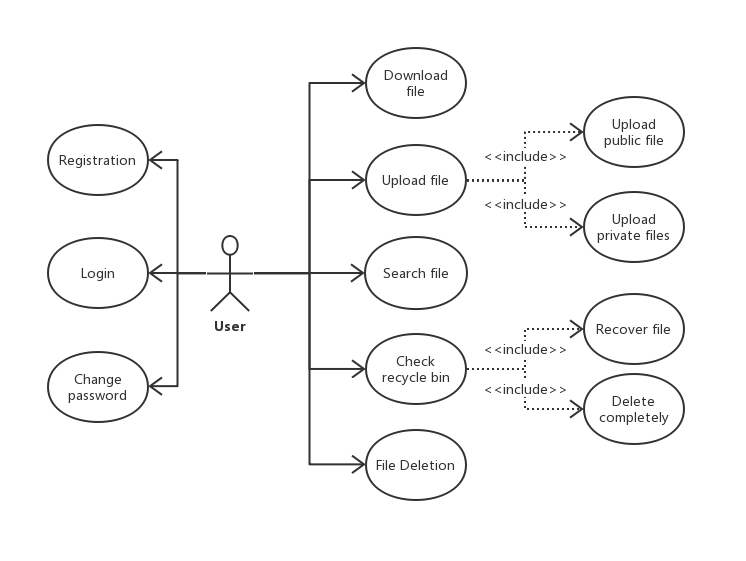
\includegraphics[scale=0.6]{Usecase.png}
\caption{Use case}
\label{fig:Usecase}
\end{figure}

\subsubsection{Design of Web Front End}
\begin{itemize}

\item \par Start page
\par There are two input text fields along with two submit button under each field at the middle of the page, which require the input of username and password respectively. After submitting registration a message would inform the user whether there is a successful or failed registration depending on formation examination (if the username is a correct email address). 
If successfully log in, jump to the home page.

\item \par Home page 
\par First part: A navigation bar on the right upper corner provide functions include changing the password, jump to recycle bin and log out. When clicking change password button a pop-out window requests old password and new password, click OK to submit, and CANCEL to close this window. Click 'recycle bin' to jump to recycle bin page and 'quit' to log out.
\par Second part: A functional bar at the middle of the page contains a search text field for searching files by user and keyword; 'clear' button for clearing current searching status; 'private space' button indicating the private file space of the current user; 'upload' button choosing the file to be uploaded.
\par Third part: File display list is designed for the existing files in the system and corresponding information including the user who uploads the file, file name and operation to the file. The user can download or delete any file visible in the public space whereas those files in private space can only be deleted by its owner.

\item \par Recycle bin page
\par This page is quite similar to the Home page. An alternative 'back' button to go back to the home page at the navigation bar is necessary. Moreover, files in the recycle bin are to be deleted permanently or recovered to where they belonged by operations at the file display list. Any operation would trigger a corresponding feedback message to show if it is executed successfully or not.
\end{itemize}

\subsubsection{Design of Android App}
\par The design of the app had been through a major modification. The app shown in the initial report had been revised to a web app as presented following. This not only solves the problem of two front-end frameworks that cannot be unified at the first stage but also improves the coding efficiency. Basically, the design of the app is very similar to the web front end.

\par A high-performance WebKit kernel browser is built into the Android system, which represents as a WebView component encapsulated in SDK. This app uses this component to display the interface of the file transfer system so that it is not constrained by the release version and can be updated in time.

\par In this app, the functions of user registration \& login, changing the password, trash bin, file deletion and recovery are all implemented on the web side. Android end only needs to load the IP address of the system to achieve all the above functions. Therefore, this app mainly focuses on the function of uploading files and downloading files to the sd card.

\subsubsection{Design of Back End}
\par The back end consists of the server and database, receiving requests from the web page or Android client and processing the requests with related functions. The server program may involve various operations related to the database, thus it is significant to use middleware to help set up connections between the server program and the database. 
\par As which is presented previously, the requirements or functions have been divided into two main types, including the user-related and file-related part. User-related part mainly contains the functions that related to users like registration, login and change the password, while the file-related part mainly focuses on the file operations like upload, download, delete and so on. The gist of partition is based on the data two types involved, which leads us that the structure of data stored in the database should also satisfy our needs.
\par Introducing the database first. Considering that there are mainly two entities involved in data management, thus we created two tables to describe two kinds of entities. One table is for user information management and the other one is for file information management. 
\par With database has been designed, a middleware is then required to provide connections between the back-end server and the database, by which it is capable for the server program to access to the database and even modify the data in the database. As for the server program, it takes charge of receiving and processing requests from the front end and call for corresponding functions to achieve the users’ goal, and send relative responses back to the front end afterwards. The detail of the back-end design will be illuminated for different functions.
\begin{itemize}
\item User login: Username and password should be transmitted within the request, which will also be passed as parameters for login function. The server will then call for a function to make a query in the database to detect whether the username and password match, sending the result back to front end.

\item User register: If a user calls for registration, username and related password will be stored in the database as completely new user information.

\item User change password: like most applications do, users need to type correctly for both old password and new password, then the server will update the password stored in the database.

\item File upload: The default location where uploaded files are stored in the public space that is available for everybody. But users could also save their files privately. Uploading involves multiple attributes including file name, user name, file content and so on. Basically, file content will be transmitted in base 64 string which will be written into the database.

\item File download: Server will receive the information of file required by the front end, then retrieve the corresponding file from the database. Send data back in base 64 string as it is uploaded. 

\item File update: This actually happens when there is already a file exist in the system with the same file name. The existed file will be replaced by newly uploaded one.

\item File delete: Files in public space can be deleted by anyone, while the private file in private space can only be deleted by the specific user. The file once has been deleted, it will be moved to trash.
Trash: Users can find every previous version of files including the files has been replaced by updating and the files have been deleted by users. Users can totally delete files in the trash, or recover the files.

\item File lock: Because of the requirement for conflict handling mechanism, a lock is introduced at this point to protecting the access of files. Basically, when a lock is gained by one user for one particular file, all other file operations will be delayed in order to protect consistency.
\end{itemize}

\section{Implementation}
% Describe the most significant implementation details, focussing on
% those where unusual or detailed solutions were required. Quote code fragments where
% necessary, but remember that the examiners have full access to your source code. Explain
% how you tested your software (e.g. unit testing) and the extent to which you tested it. If
% relevant to your project, explain performance issues and how you tackled them.
\subsection{Implementation of Web Front End}
\begin{itemize}
\item Start page (start.html)

\begin{figure}[ht]
    \centering
    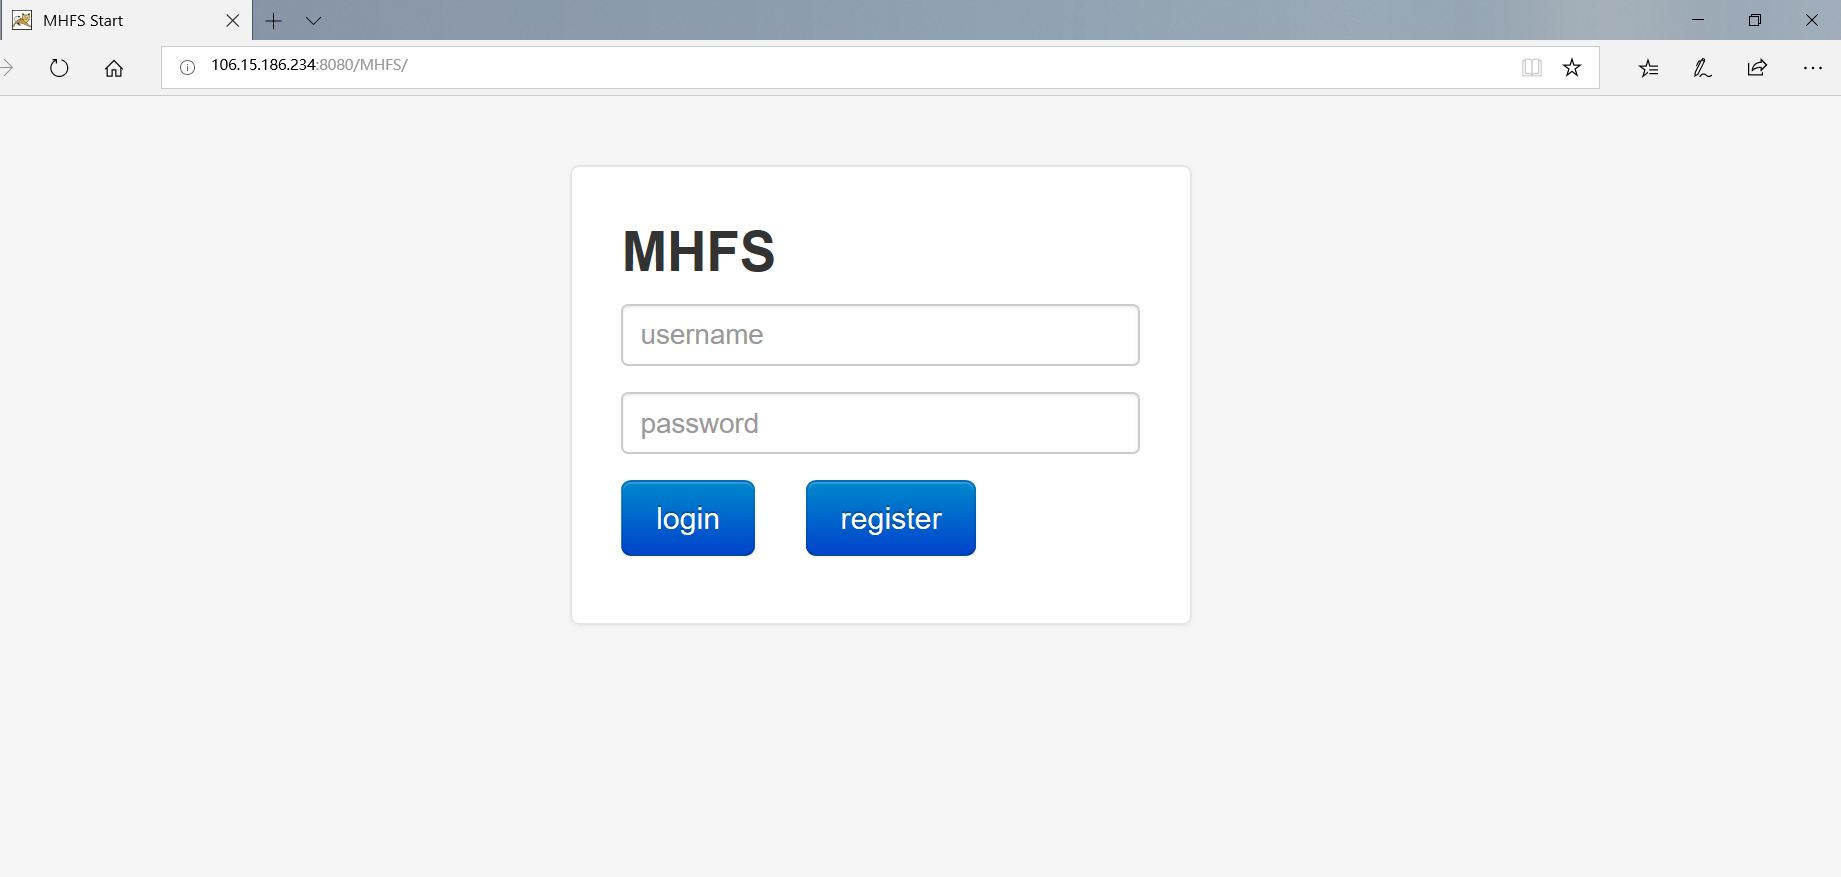
\includegraphics[scale=0.3]{1p.png}
    \caption{Start page}
    \label{fig:Start page}
\end{figure}
\par Registration: After input username and password, click 'register' button and the method registerAction() in {$\langle$}script{$\rangle$} will be invoked by onclick property. The logic of registerAction() is that first check if the formation of the username is correct and not empty by checkValue(). If the return value is true then create JSON object and obtain username and password from the page by jQuery in order to assign them to a JSON object. A post request over HTTP is sent to StartServlet where the action is registered along with a JSON object. Afterwards, the StartServlet returns a JSON-formatted string (JSON string for short) to method registerAction(), then it converts the JSON string into a JSON object and determines its ret property. If ret = 0, the registration is successful (a popup window prompts for success) and the start page is reloaded while the user can log in with his registered user name. If ret = 1, registration fails (a popup window prompts failure).
\par Login: Once the username and password have been input, clicking the Login button triggers the method in {$\langle$}script{$\rangle$} through the onclick property: loginAction(). Similarly, a post request over HTTP is sent to StartServlet where the action is login now. The StartServlet also returns a JSON string after processing. Judge ret value after converting to a JSON object. If ret = 0, skip to home.html. Otherwise, login fails (popup window prompts failure).

\item Home page (home.html \& home.js)
\begin{figure}[ht]
    \centering
    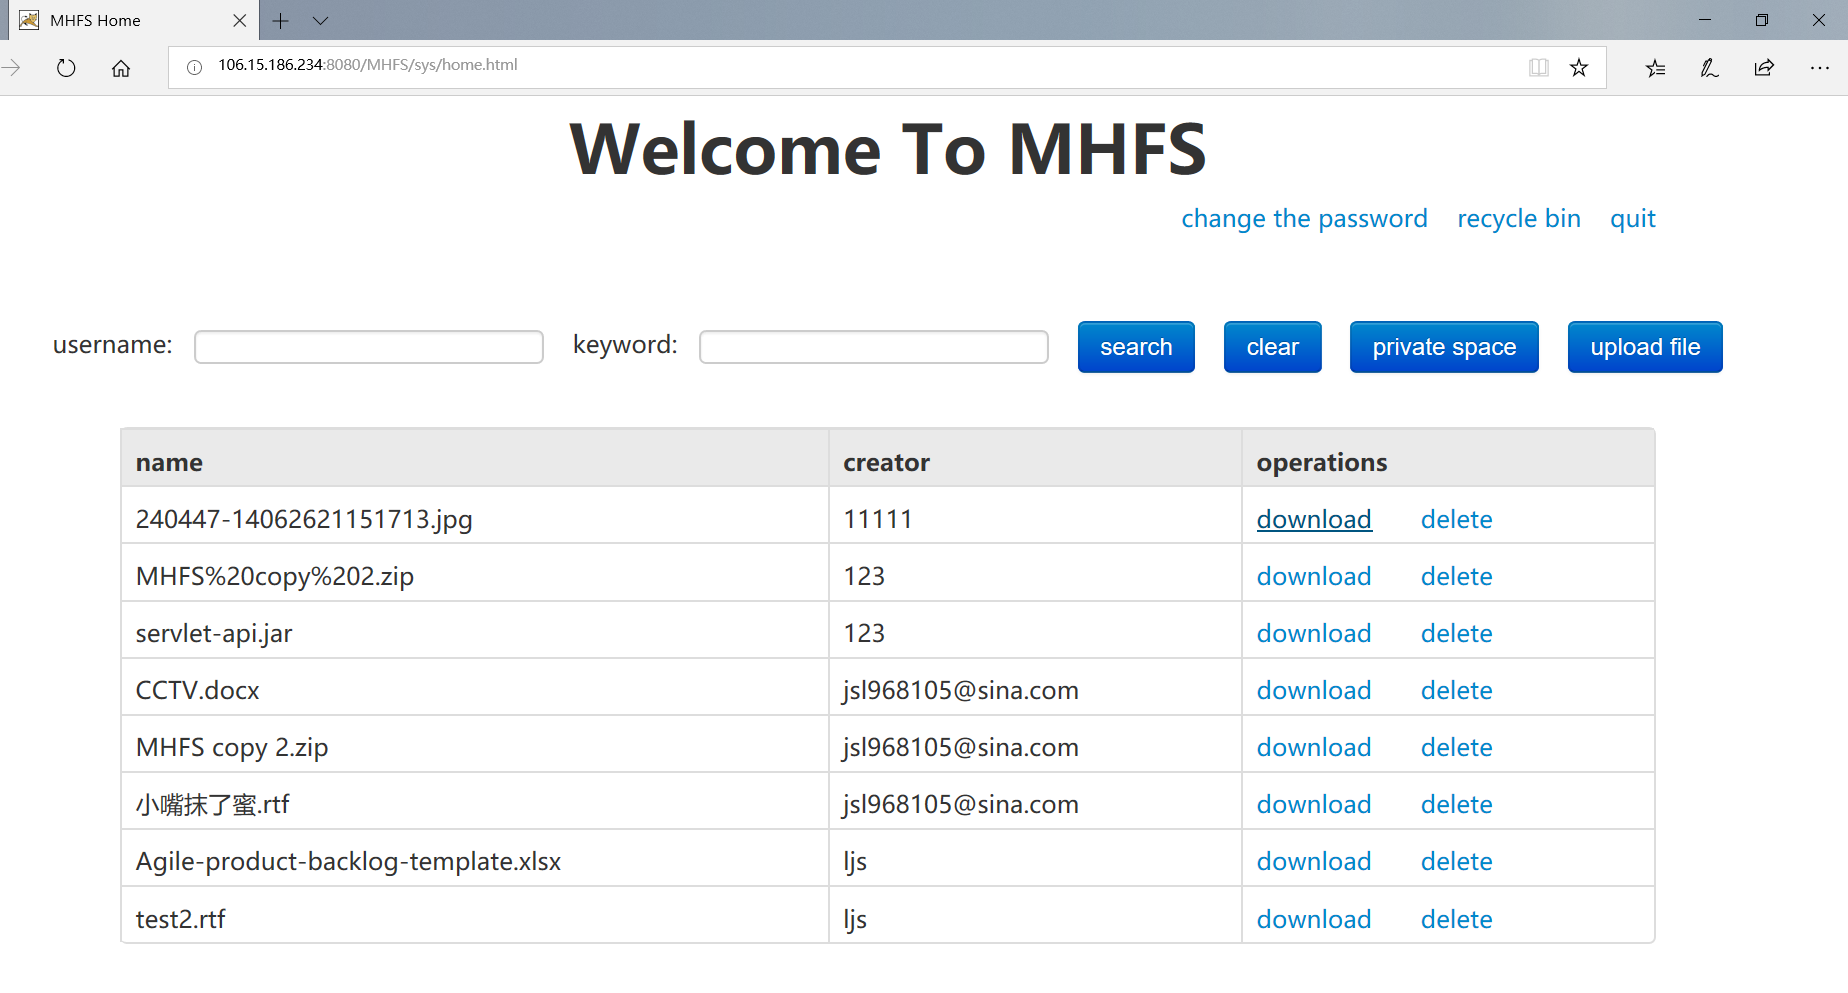
\includegraphics[scale=0.3]{2p.png}
    \caption{Home page}
    \label{fig:Home page}
\end{figure}

\par Logic of change password and upload file are contained in {$\langle$}script{$\rangle$}.

\begin{figure}[ht]
    \centering
    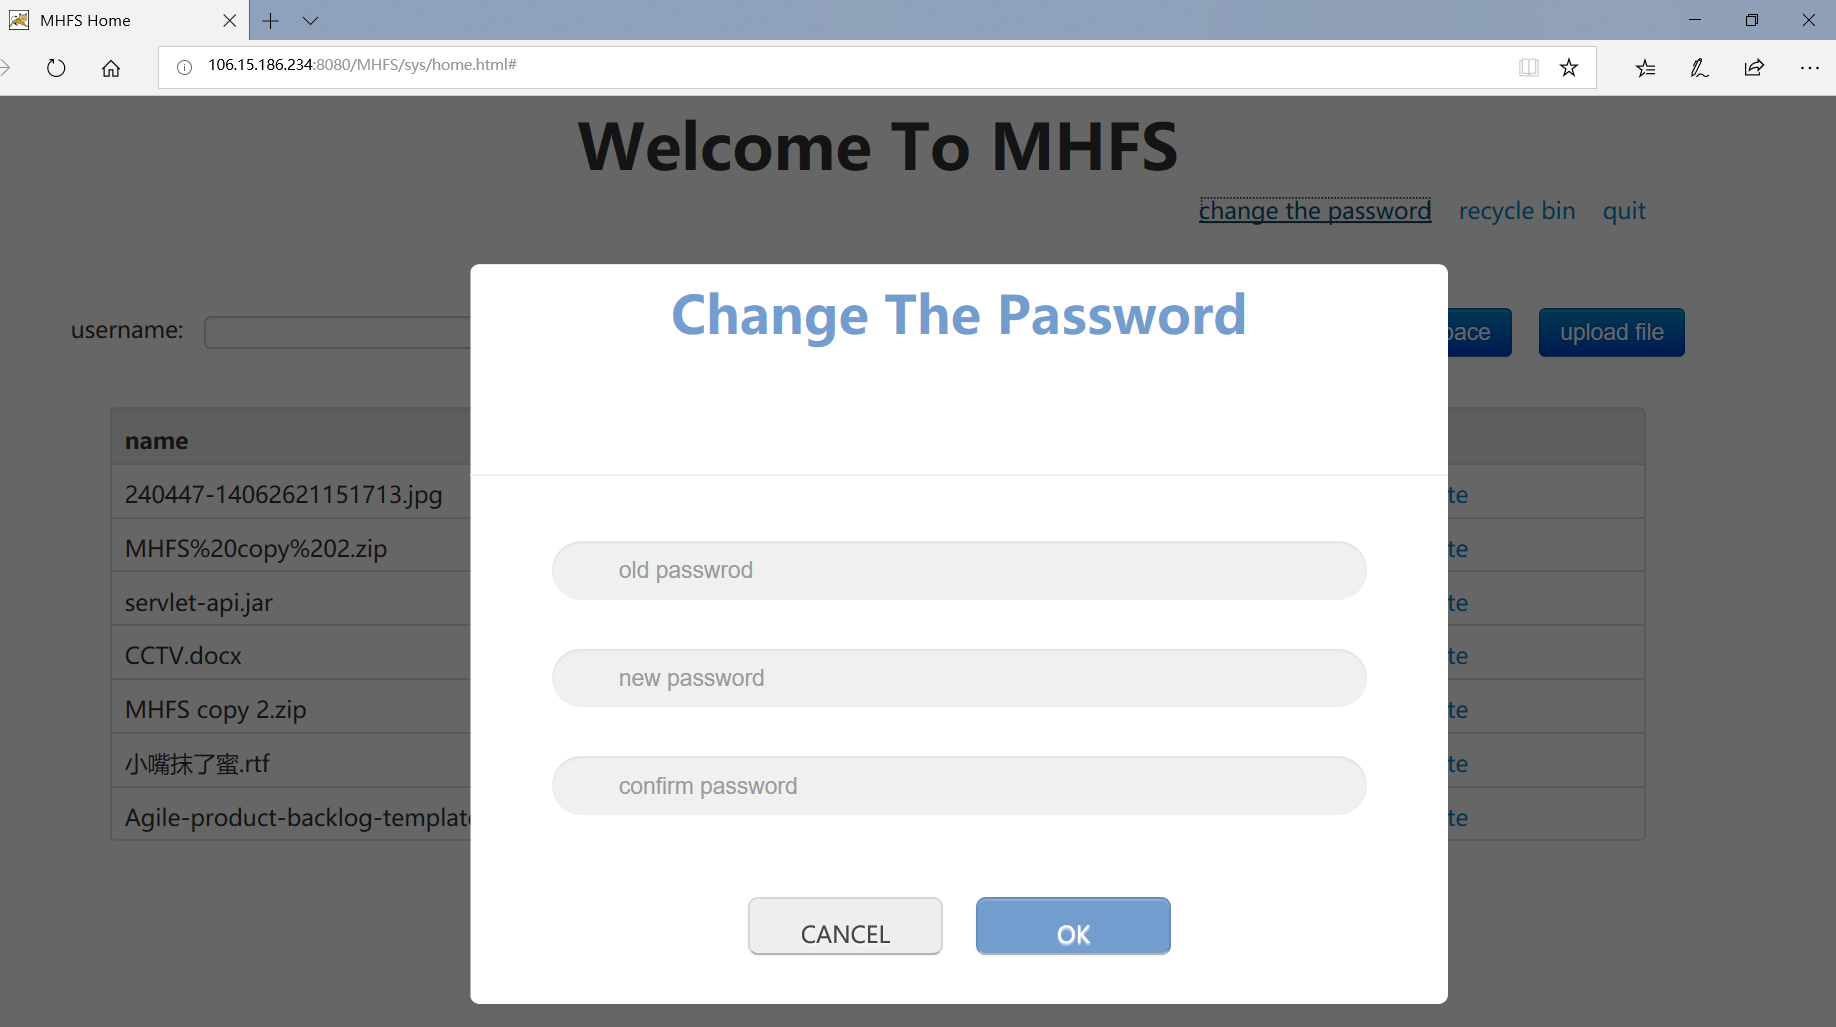
\includegraphics[scale=0.3]{3p.png}
    \caption{Change password}
    \label{fig:Change password}
\end{figure}

\par Change password: Click method is triggered by acquiring the jQuery object where the name is 'changePwd'. Click method indicates {$\langle$}div{$\rangle$} of class = mypop through its anonymous function and empty all the value of password fields by \$(":password").val(' '). Then modify the rendering of the password window.
Click CANCEL to hide the object by taking the jQuery object with name = CANCEL and class = close and calling the hide() method of the jQuery object with class = mypop through the anonymous function in the click. Clicking 'OK' after entering a username and password triggers the changePwd() method. The logic of changePwd() is to take the values of the three password boxes. First, determine whether it is non-null and the new password values entered twice match. If true then create a JSON object and set the properties 'op' and 'np' and their corresponding values. The JSON object is sent to the UserServlet via an HTTP post request where the action is changePwd. Then the UserServlet returns a JSON string, which is converted to a JSON object to determine the ret property value. If ret = 0 then the password is successfully changed and a popup window gives the user feedback. Otherwise, it fails.

\par Recycle bin: Click the hyperlink to jump directly to trash.html.

\par Quit: Click on the hyperlink to call method quit() which sends the HTTP post request to the UserServlet (action = quit). The UserServlet returns a JSON string, which is converted to a JSON object by this method to determine the value of ret property. If ret=0, log out succeeds and jump to start.html. Otherwise, logout fails.

\par The above is JavaScript code to achieve several functions in the home.html page. The rest of the JavaScript code is written separately from the home.js file and embedded in the home.html. This is because the remaining various functions are related to files, and should be executed after the complete loading of the file display list, thus the first line of home.js code '\$(document).ready(search);' indicates that the search method is to be executed automatically after the page loads.

\par Search and file display list: The search() method takes the value in the tags with name = username and keyword, assigns the value to the JSON object, and sends the FileServlet (action = search) with an Http post request. The FileServlet calls the show() method after the returned JSON string is converted to a JSON object. Show() takes an element with an id of the tab and write it into an HTML statement. This statement helps create a table at the page with column elements name, creator and operations. The for loop output the filename and the creator, bounded by the length attribute of the JSON object. Meanwhile, set both links for download and delete. At the end of the loop, the file list output is complete. Click the private space button to invoke the priSearch() method. Send HTTP post request to FileServlet (action = priSearch) after setting flag = 2. After getting the JSON string returned by the FileServlet and transferring it into a JSON object, make the variable pri=1 and call the show() method.

\begin{figure}[ht]
    \centering
    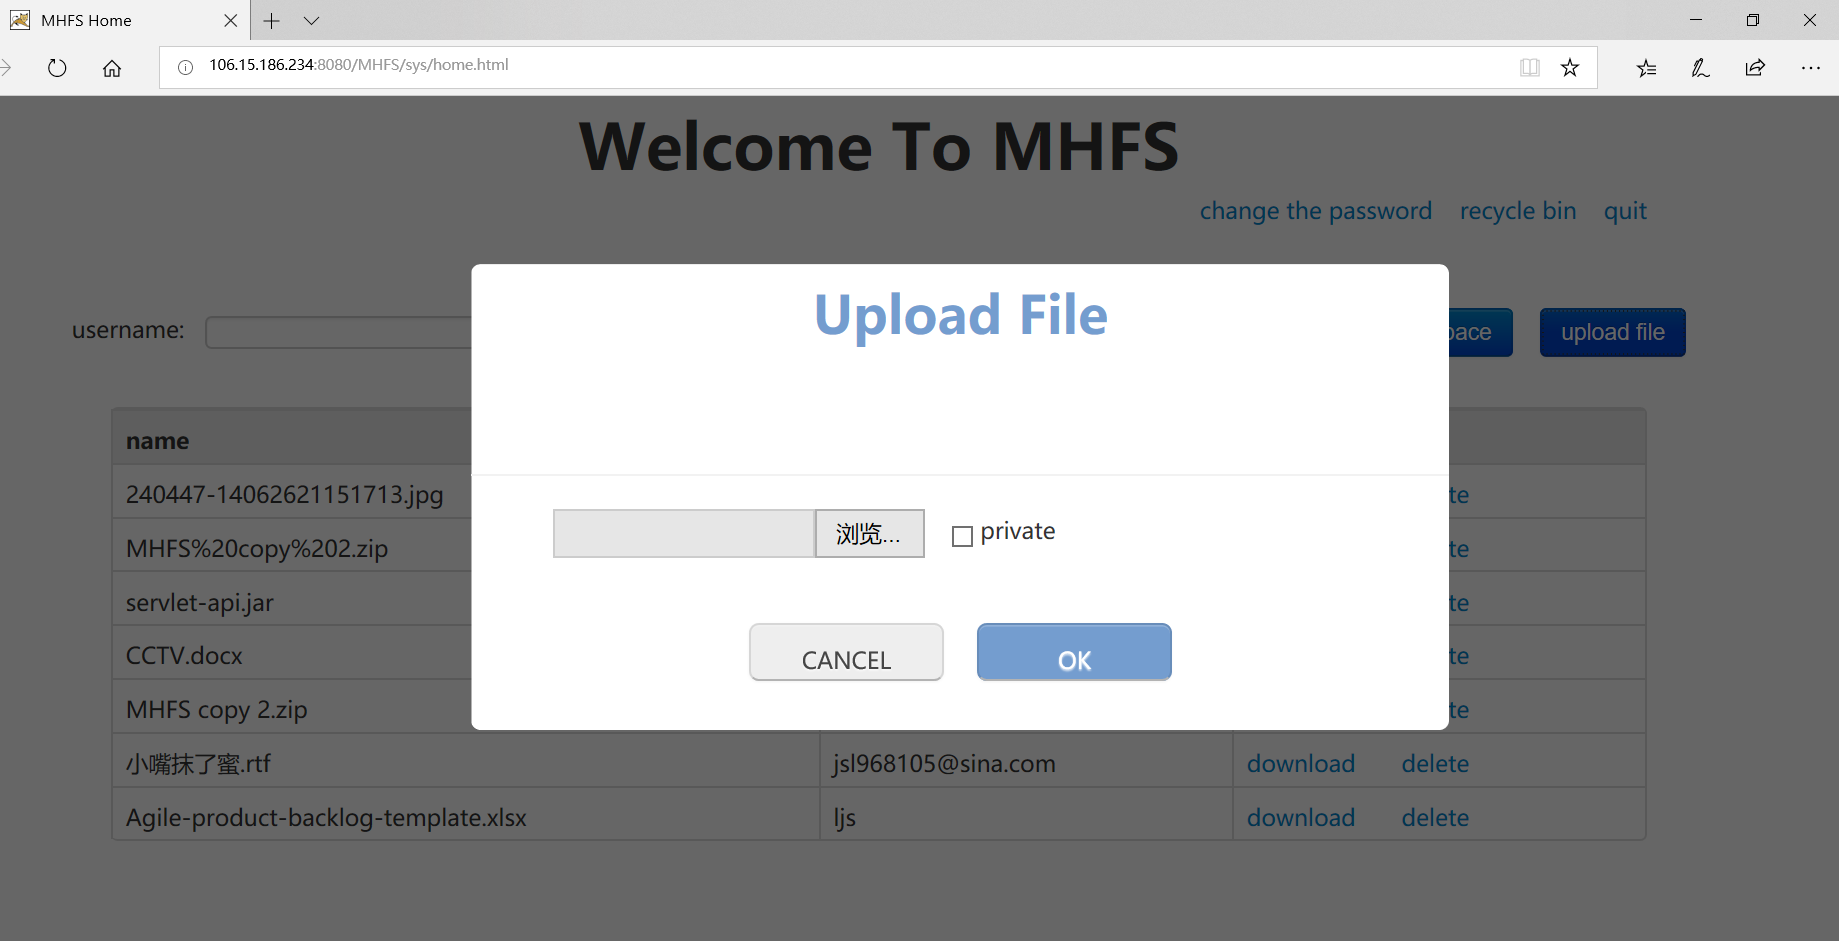
\includegraphics[scale=0.3]{4p.png}
    \caption{Upload file}
    \label{fig:Upload file}
\end{figure}

\par Upload: Click the 'uploadfile' button to trigger the click event so that the tag of (class = upload) is showed, which is the file transfer interface. After selecting the file to upload, a reader object is created by the FileReader class in the web API when selecting the file due to the use of a change method of jQuery. The reader object reads the file selected by the user and uses the 'onload' attribute to write the contents of the file to a jQuery object with id file\_base64 by triggering a load event. After that, click the "OK" button to trigger the onclick event to invoke method upload(). Method upload() will first check whether the value of the jQuery object with id = fileup is 'undefined' or null. If not then continue to check whether the check box is selected, if selected then this is a personal file (pri = 1), otherwise a public file (pri = 0). Next, divide the value of this jQuery object by method split() and assign the result to parameter 'Business' which is an Object Array. The last element of the array is the name of the file uploaded. Assign this file name to parameter 'fileName' and use string fileName as the URI. Additionally, in order to prevent unreadable code, the string is encoded by encodeURI function. Create JSON object and assign its properties fname, fcontent and pri respectively.
Send the FileServlet an HTTP post request (action = upload) and send the JSON object to the server. After the JSON string returned by the server is converted into a JSON object, the ret value of its attribute is checked. If ret = 0, the modification is successful (popup indicates success), hide the file upload interface and redisplay the updated file list. Otherwise, the upload fails (popup prompts failure).

\begin{lstlisting}[language=Java]
function upload() {
	if($("#fileup").val() == undefined || $("#fileup").val() == ""){
		return;
	}
	var pri = 0;
	if($('#cx').prop('checked')){
		pri = 1;
	}
	var Business = $("#fileup").val().split("\\");
	var fileName =  Business[Business.length-1]
	fileName = encodeURI($("#fileup").val());
	var json={ "fname" : fileName, "fcontent" : $("#file_base64").val(), "pri" : pri};
	$.post("../system/FileServlet?action=upload", json, function(data) {
		var obj = JSON.parse(data);
		if(obj.ret === "0"){
			alert("file upload successfully");
			 $('.uploadfile').hide();
			if(pri == 0) {
				search();
			} else {
				priSearch();
			}
		} else {
			alert(obj.msg);
		}
	});
}
\end{lstlisting}

\par Download: Click the 'download' button to trigger click event and call the method down(). Gets the class name (int) of the current tag, and the value of the class gives the file name of the current line. Assign filename and pri to the JSON object and send the HTTP post request (action = download) and JSON object to the FileServlet. After converting the FileServlet's JSON string into a JSON object, create a jQuery object of tag {$\langle$}a{$\rangle$}. Determine the ret attribute value of the JSON object. If ret=0, make the href = encode URI (file content) in tag {$\langle$}a{$\rangle$}. Set the style of tag {$\langle$}a{$\rangle$} as hidden, download attribute value = file name. Attach the tag {$\langle$}a{$\rangle$} to the web page and trigger its click event before deleting it. The file download is complete. If ret = 1, the download fails (popup prompts failure).

\begin{lstlisting}[language=Java]
function down(source){
	var className = source.getAttribute("class");
	var name =  document.getElementById("tab").rows[parseInt(className) + 1].cells[0].innerHTML;
	
	var json={"fname" : name , "pri" : pri};
	console.log("pri: "+json);
	$.post("../system/FileServlet?action=download", json, function(data) {
		var obj = JSON.parse(data);
		var link = document.createElement("a");
		if(obj.ret=="0"){
			link.href = encodeURI(obj.fContent);
			link.style = "visibility:hidden";
        	link.download = obj.fName;
        	document.body.appendChild(link);
        	link.click();
        	document.body.removeChild(link);

		}
		else{
			alert(obj.msg);
		}
       
	});
}
\end{lstlisting}

\par Delete: Click 'delete' button to trigger the click event and invoke the method del(). Gets the class name (int) of the current tag, and the value of the class gives the file name of the current line. Assign filename and pri to the JSON object and send the HTTP post request (action = delete) and JSON object to the FileServlet. After converting the JSON string returned by the FileServlet into a JSON object, the ret property value of the JSON object is determined. If ret = 0, delete successfully (popover indicates success). If flag = 1, then call search() and call priSearch() if flag=2. If ret = 1, the deletion fails (popover prompts failure).

\item Recycle bin page (trash.html \& trash.js)

\begin{figure}[ht]
    \centering
    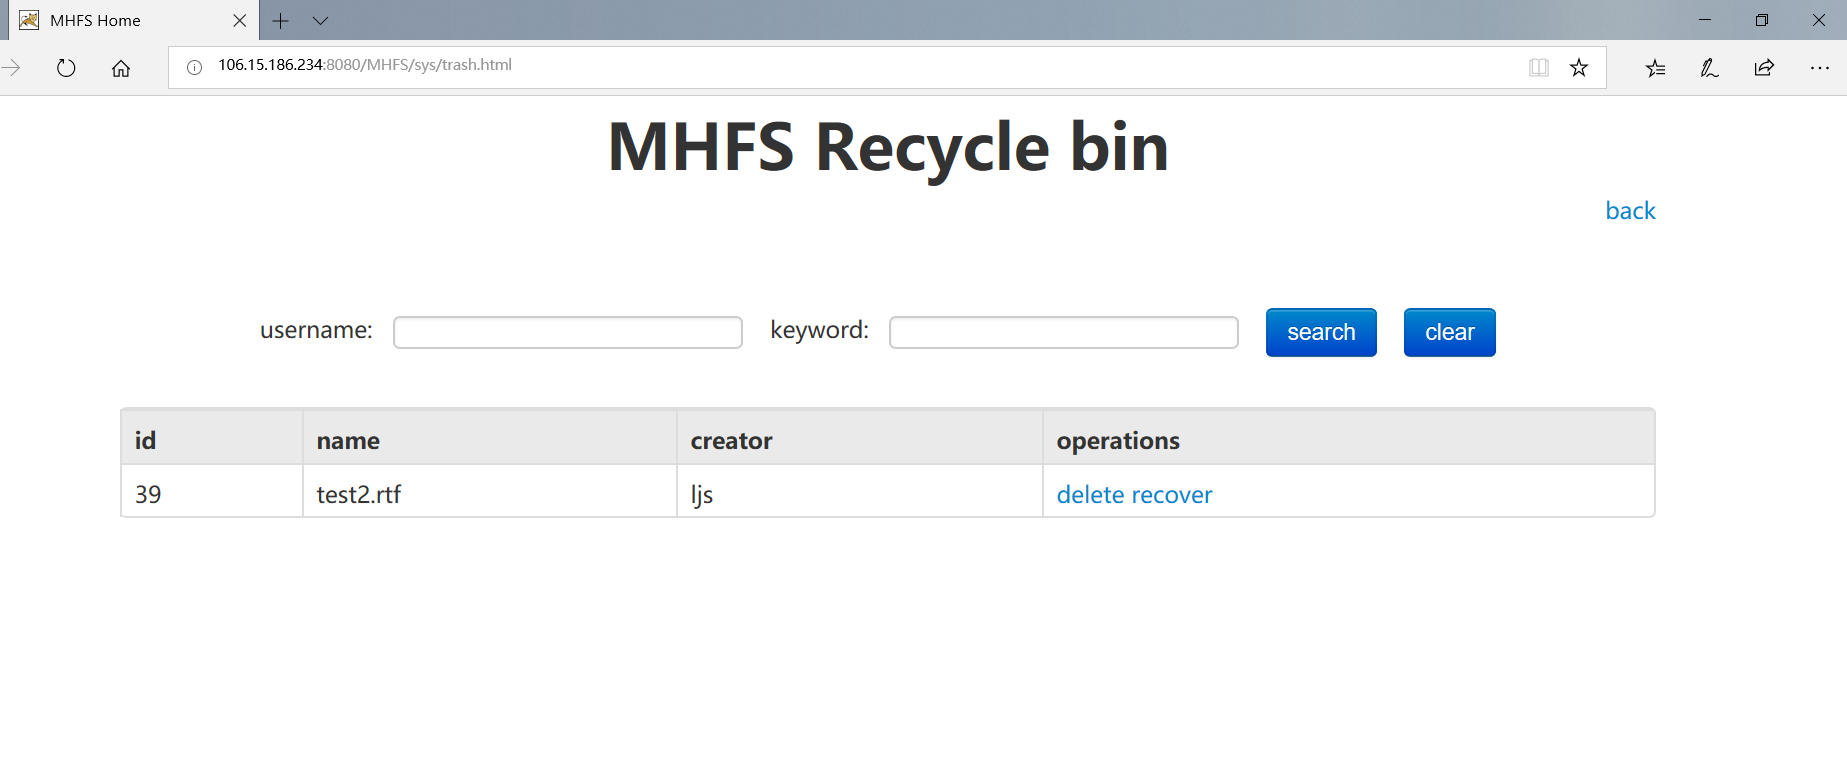
\includegraphics[scale=0.3]{5p.png}
    \caption{Recycle bin page}
    \label{fig:Recycle bin page}
\end{figure}

\par The search function is the same as the home page. New functions for file recovery and complete deletion are added.

\par Complete deletion: Clicking the 'delete' button triggers the click event and invokes the method totalDel(). 
Gets the class name (int) of the current tag, and the file id of the current line can be obtained by the value of the class. Assign the id to the JSON object and then send the HTTP post request (action = totallyDelete) and JSON object to the FileServlet. After converting the JSON string returned by the FileServlet into a JSON object, the ret property value of the JSON object is determined. If ret = 0, delete successfully (popup window indicates success). If flag = 1, then call search() while call priSearch() if flag=2. If ret = 1, the deletion fails (popover prompts failure).

\par Recovery: Click the 'recover' button to trigger the click event and invoke recover(). Recover() logic: retrieves the class name (int) of the current tag, and the value of the class provides the file name and id of the current line. After assigning the file name, pri and id to the JSON object, send HTTP post request (action = recover) and JSON object to the FileServlet. After converting the JSON string returned by the FileServlet into a JSON object, the ret property value of the JSON object is determined. If ret = 0, the recovery is successful (popover indicates success). If flag = 1, search() is called. Otherwise, the recovery fails (popover prompts failure).

\end{itemize}

\subsection{Implementation of Android App}
\par Since only the implementation of upload and download are different from the web side, it is necessary to write a new method for the system to complete these two functions. 
\par The WebView class is the view class of the Java layer of the WebKit module. All Android applications that need to use the Web browsing capability create this view object to display and process the requested network resources. Currently, the WebKit module supports HTTP, HTTPS, FTP, and javascript requests. As the UI interface of the application, WebView provides users with a series of web browsing and user interaction interfaces through which the client program can access the core WebKit code.
\par The Android front end of this group, by configuring network permissions, uses the load method to load the URL while loading the activity and displays the Web page corresponding to the URL. By setting the WebViewClient for the WebView, the page is displayed inside the App. More importantly, with setJava ScriptEnabled(true), Android uses js in WebView and through mWebview.loadUrl(" ")
to enable the interaction between Android and JavaScript. In addition, Android uses shouldOverrideUrlLoading function to redirect the URL to implement trigger.
\par Override the onKeyDown method on the outside of the onCreate function to provide the key response function. When viewing the web page in the WebView, press the return button to return by browsing history. If this is not done, the whole WebView will return and exit. Through interaction, all functions of the web side can be realized within the Android App. In order to adapt to various Android models, WebChromeClient subclass has added methods for Android 3.0+, 4.1, 5.0+ Lollipop (SDK 22) to upload pictures from the local selection.

\begin{itemize}
    \item Upload
    \par Since uploading files to the server requires some methods on the Android front end to receive parameters or data from the back end, set WebChromeClient subclass in the Activity.
    \par Take android device version 5.0+ as an example, click the choose file button to call the onShowFileChooser file selector method, and add the judgment whether the uploaded file is empty or not. If it is not empty, then determine uploadMessage = filePathCallback to select the image path and return the Uri[I] type value to the jquery object. Use implicit page jump to open the local file. If the jump fails, notification will be toasted to the activity of the App.
    
    \begin{lstlisting}[language=Java]
      public boolean onShowFileChooser(WebView mWebView, ValueCallback<Uri[]> valuecb, WebChromeClient.FileChooserParams params)
    {
        if (upload != null) {
            upload.onReceiveValue(null);
            upload = null;
        }

        upload = valuecb;

        Intent intent = params.createIntent();
        try
        {
            startActivityForResult(intent, REQUEST_SELECT_FILE);
        } catch (ActivityNotFoundException e)
        {
            upload = null;
            Toast.makeText(getBaseContext(), "Cannot Open File Chooser", Toast.LENGTH_LONG).show();

            return false;
        }
        return true;
    }
    \end{lstlisting}
    \newpage
    \item Download
    \par Slightly different from the upload function, The download involves an API, ContextCompat.checkSelfPermission, being used outside of onCreate function. 
    
    \begin{lstlisting}[language=Java]
    public static boolean checkPermissions(Context context, String... permissions) {
        if (Build.VERSION.SDK_INT >= Build.VERSION_CODES.M && context != null && permissions != null) {
            for (String permission : permissions) {
                if (ContextCompat.checkSelfPermission(context, permission) != PackageManager.PERMISSION_GRANTED) {
                    return false;
                }
            }
        }
        return true;
    }
    \end{lstlisting}
    
    \par This is mainly used to detect whether certain permission has been granted. The return value of this method is PackageManager.PERMISSION\_DENIED or PackageManager.PERMISSION\_GRANTED. It is necessary to apply for permission when the return value is DENIED. Then use the asynchronous method ActivityCompat.RequestPermissio\-ns(thisActivity, new String[]\{the Manifest.Permission.READ\_CONTACTS\}, MY\_PERM\-ISSIONS\_REQUEST\_READ\_CONTACTS) to apply for the permission, where requestCode are mainly responsible for the testing when callback, then pass requestCode into the callback function onRequestPermissionsResult for the next operation.
    
    \begin{lstlisting}[language=Java]
    if (!checkPermissions(MainActivity.this,new String[]{Manifest.permission.WRITE_EXTERNAL_STORAGE})){
        // Permission ask
            ActivityCompat.requestPermissions(MainActivity.this, new String[]{Manifest.permission.WRITE_EXTERNAL_STORAGE}, 111);
            Log.e("permission","Ask for permission");
        } else {
        // if permission is already granted than load url
            downloadUrl();
        }
    \end{lstlisting}
    
    \par For the result of the permission application, first, verify the requestCode and locate the application to that permission, then verify that grantResults corresponds to the result of the application. 
    
    \begin{lstlisting}[language=Java]
    @Override
    public void onRequestPermissionsResult(int requestCode, String[] permissions, int[] grantResults) {
        super.onRequestPermissionsResult(requestCode, permissions, grantResults);

        if (requestCode == 111) {
            //i guess maybe the value pf grantresults has never been changed
            if (grantResults.length > 0 && grantResults[0] == PackageManager.PERMISSION_GRANTED) {
                downloadUrl();
            } else {
                //actually when download is happens it just went through all the permissioncheck flow to this toast ,i just don't know why
                Toast.makeText(MainActivity.this, "The app was not allowed to read your storage.", Toast.LENGTH_LONG).show();
            }
        }
    }
    \end{lstlisting}
    
    \par If the application is successful, the downloadURL (the download method) is executed. Within the method, the webView's download listening is activated. At this point, the download event is successfully triggered.
    \par Click the download button to trigger the click event and invoke the WebView download listener method within the downloadURL. In the overridden function onDownloadStart, use the Android built-in DownloadManager  to handle Http/Https connections and monitor status changes and system restarts to ensure that each download task completes successfully. Due to the character accepted by the system is encoded as base64 in the JSON object, and cannot be used by DownloadManager.Request. Therefore, processing the received parameter by attaching the HTTP prefix to ensure that the download event is processed correctly.

    \begin{lstlisting}[language=Java]
    public void downloadUrl() {

         mWebview.setDownloadListener(new DownloadListener() {

             public void onDownloadStart(String url, String userAgent, String
                     contentDisposition, String mimetype, long contentLength) {

                 Log.e("DOWNLOAD", "Permission Granted");

                 //change from base64 to http string ,need double check with Fei& LJS
                 String dlurl = "http://106.15.186.234/MHFS/sys/home.html\n" + url;
                 DownloadManager.Request request = new DownloadManager.Request(Uri.parse(dlurl));
                 request.setMimeType(mimetype);
                 request.addRequestHeader("User-Agent", userAgent);
                 String filename = URLUtil.guessFileName(dlurl, null, null);
                 request.setTitle(filename);
                 request.allowScanningByMediaScanner();
                 request.setNotificationVisibility
                 (DownloadManager.Request.VISIBILITY_VISIBLE_NOTIFY_COMPLETED);
                 //define a new file in phone storage 
                 request.setDestinationInExternalPublicDir
                 (Environment.DIRECTORY_DOWNLOADS, filename);
                 DownloadManager dm = (DownloadManager) getSystemService(DOWNLOAD_SERVICE);
                 dm.enqueue(request);

                 Toast.makeText(MainActivity.this, "Download Successful", Toast.LENGTH_LONG).show();
             }
         });
     }
    \end{lstlisting}
\end{itemize}
\subsection{Database}
\subsubsection{Version and Environment}
\par To ensure data reliability and security, we used MySQL Server 5.7 + MySQL Workbench 8.0 to deploy and manage database systems, use SQL's own data backup and security guarantee to support data security for this project. Our database system runs on the remote Alibaba Cloud server, providing services 24/7, and opening the 3306 interface for remote management access. The database administrator can use the root account to remotely manipulate the database system.
\subsubsection{Logical Design (E-R Diagram)}

\par We refer to “Database System implementation” to standardize the naming of database parameters and normalize the structure of the table to satisfy the third paradigm, The Entity-relationship model is as follows.

\begin{figure}[ht]

\centering
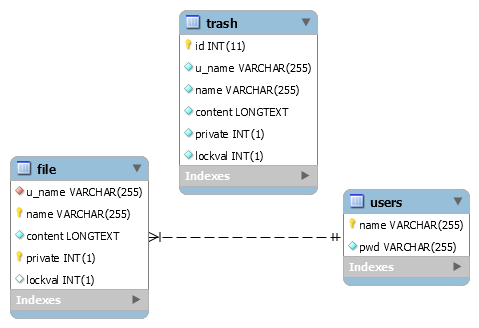
\includegraphics[scale=0.6]{SQL-E-R.png}
\caption{SQL E-R diagram}
\label{fig:SQL E-R}
\end{figure}

\subsubsection{Physical Design}

\begin{table}[H]
\centering
\setlength{\tabcolsep}{1.5mm}{
\begin{tabular}{|c|c|c|c|c|c|p{3cm}|}
\hline
\multicolumn{2}{|c|}{Table Name} & \multicolumn{5}{|c|}{Users}\\
\hline
\multicolumn{2}{|c|}{Table User} & \multicolumn{5}{|c|}{Admin \& Backend application}\\
\hline
\multicolumn{2}{|c|}{Primary key} & \multicolumn{5}{|c|}{name}\\
\hline
\multicolumn{2}{|c|}{Index} & \multicolumn{5}{|c|}{Null}\\
\hline
ID & Column name & Data type & Not null & Unique & Default value & constraint \\
\hline
1 & Name & VARCHAR(255) & YES & YES & NULL & Primary key \\
\hline
2 & Pwd & VARCHAR(255) & YES & NO & NULL & \\
\hline
\multicolumn{2}{|c|}{SQL script} & \multicolumn{5}{|p{12cm}|}{\tabincell{c}{CREATE TABLE`users`(\\
`name` varchar(255) NOT NULL,
\\`pwd` varchar(255) NOT NULL,
\\PRIMARY KEY(`name`))}}\\
\hline
\multicolumn{2}{|c|}{Description} & \multicolumn{5}{|p{12cm}|}{User table used to store user information (username and password), the user name is the primary key, neither is allowed to be null}\\
\hline

\end{tabular}}
\caption{Physical design-1}
\end{table}






\begin{table}[H]
\centering
\setlength{\tabcolsep}{1.5mm}{
\begin{tabular}{|c|c|c|c|c|c|p{3cm}|}

\hline
\multicolumn{2}{|c|}{Table Name} & \multicolumn{5}{|c|}{File}\\
\hline
\multicolumn{2}{|c|}{Table User} & \multicolumn{5}{|c|}{Admin \& Backend application}\\
\hline
\multicolumn{2}{|c|}{Primary key} & \multicolumn{5}{|c|}{name \& private as joint primary key}\\
\hline
\multicolumn{2}{|c|}{Index} & \multicolumn{5}{|c|}{Null}\\
\hline
ID & Column name & Data type & Not null & Unique & Default value & constraint \\
\hline
1 & u\_name & VARCHAR(255) & YES & NO & NULL & \\
\hline
2 & name & VARCHAR(255) & YES & YES & NULL & Primary key\\
\hline
3 & content & LONGTEXT & YES & NO & NULL & Files base64 content\\
\hline
4 & private & INT(1) & YES & NO & 0 & Value=1 when file is private, Value=0 when file is public \\
\hline
5 & lockval & INT(1) & YES & NO & 1 & Value=1 when file is locked, other process blocked \\
\hline
\multicolumn{2}{|c|}{SQL script} & \multicolumn{5}{|p{12cm}|}{\tabincell{c}{CREATE TABLE `file` (\\
  `u\_name` varchar(255) NOT NULL,\\
  `name` varchar(255) NOT NULL,
  `content` longtext NOT NULL,\\
  `private` int(1) NOT NULL,
  `lockval` int(1) DEFAULT '1',\\
  PRIMARY KEY (`name`,`private`),
  KEY `username\_idx` (`u\_name`),\\
  CONSTRAINT `username` FOREIGN KEY (`u\_name`) \\
  REFERENCES `users` (`name`) \\
  ON DELETE NO ACTION ON UPDATE NO ACTION)
}}\\
\hline
\multicolumn{2}{|c|}{Description} & \multicolumn{5}{|p{12cm}|}{file table used to store files’ attributes and content, the combination of name and private is the primary key, column content stores file’s base64 content, field lockval record whether the file is being used, thereby avoiding access violations }\\
\hline

\end{tabular}}
\caption{Physical design-2}
\end{table}


\begin{table}[H]
\centering
\setlength{\tabcolsep}{1.5mm}{
\begin{tabular}{|c|c|c|c|c|c|p{3cm}|}

\hline
\multicolumn{2}{|c|}{Table Name} & \multicolumn{5}{|c|}{Trash}\\
\hline
\multicolumn{2}{|c|}{Table User} & \multicolumn{5}{|c|}{Admin \& Backend application}\\
\hline
\multicolumn{2}{|c|}{Primary key} & \multicolumn{5}{|c|}{id}\\
\hline
\multicolumn{2}{|c|}{Index} & \multicolumn{5}{|c|}{Null}\\
\hline
ID & Column name & Data type & Not null & Unique & Default value & constraint \\
\hline
1 & id & INT(11) & YES & YES & NULL & Primary key\\
\hline
2 & u\_name & VARCHAR(255) & YES & NO & NULL & \\
\hline
3 & name & VARCHAR(255) & YES & NO & NULL & \\
\hline
4 & content & LONGTEXT & YES & NO & NULL & Files base64 \\
\hline
5 & private & INT(1) & YES & NO & 0 & Value=1 when file is private, Value=0 when file is public \\
\hline
6 & lockval & INT(1) & YES & NO & 0 & Value=1 when file is locked, other process blocked\\
\hline
\multicolumn{2}{|c|}{SQL script} & \multicolumn{5}{|p{12cm}|}{\tabincell{c}{CREATE TABLE `trash` (\\
  `id` int(11) NOT NULL AUTO\_INCREMENT,\\
  `u\_name` varchar(255) NOT NULL,\\
  `name` varchar(255) NOT NULL,\\
  `content` longtext NOT NULL,\\
  `private` int(1) NOT NULL,\\
  `lockval` int(1) NOT NULL DEFAULT '0',\\
  PRIMARY KEY (`id`))
}}\\
\hline
\multicolumn{2}{|c|}{Description} & \multicolumn{5}{|p{12cm}|}{Same as file table, column content stores file’s base64 content, field lockval record whether the file is being used, thereby avoiding access violations}\\
\hline

\end{tabular}}
\caption{Physical design-3}
\end{table}



\subsection{Implementation of Back End}

\par The back-end server is mainly implemented by JAVA EE, which connects to Oracle Mysql database with JDBC to enable JAVA programs to operate on SQL database.

\par About the implementation of the file lock mechanism: Inspirited by the most primitive mutex and the concept of semaphore, define a file attribute called lockval, this attribute is like a flag by which the system can determine whether to request a lock. When a process wants to lock a particular file, it needs to check the lockval attribute of the file first. If this flag is 0, it means that there is no lock and no other user is operating the file at the moment, then the process can request to acquire a file lock and set its file to lock state i.e. let lockval = 1. If lockval is 1, it indicates that the current file is being locked due to operation by some other process. Thus the process cannot acquire the lock and can only passively wait for the end of the operation and release of the lock. This is one of most basic bottom implementation methods for the locking mechanism. The reason of choosing this method instead of the encapsulated method, such as the lock mechanism in Java is that although this way may seem to be more complex, it has strong controllability and allows developers to make adjustments to the greatest extent.

\begin{figure}[ht]

\centering
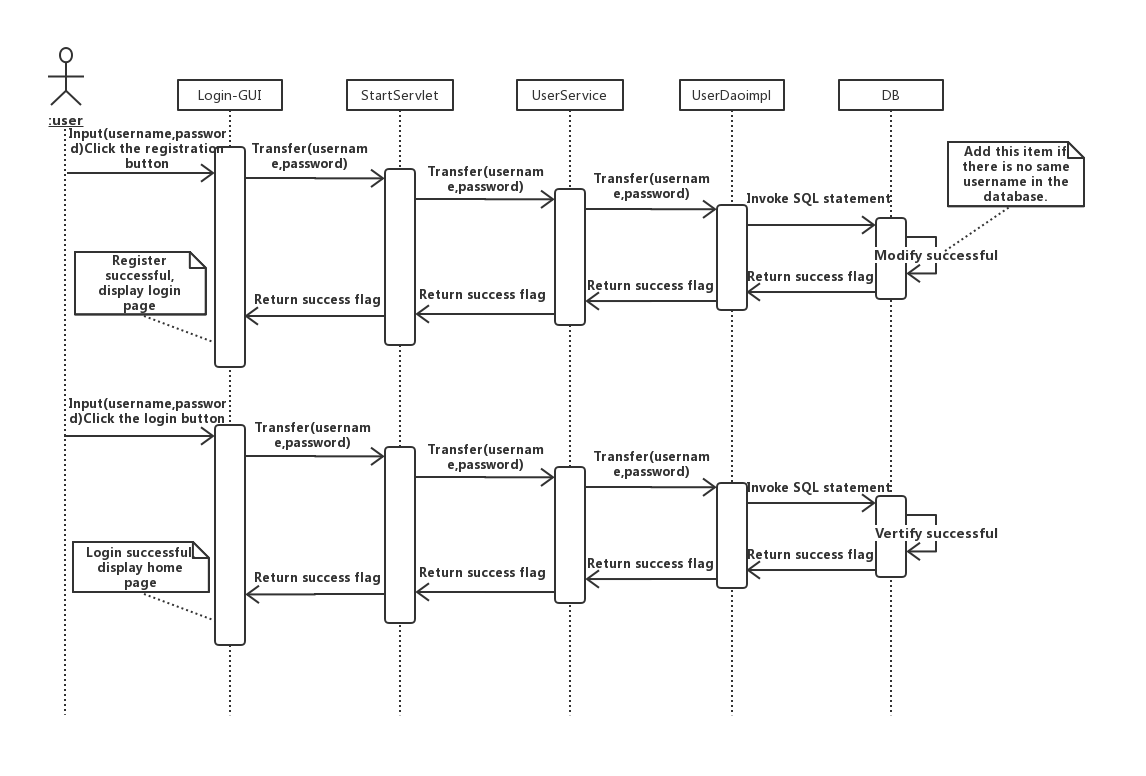
\includegraphics[scale=0.39]{Sequence_diagram_register_and_login.png}
\caption{Sequence diagram of register and login}
\label{fig:Sequence diagram of registration and login}
\end{figure}

\begin{figure}[ht]

\centering
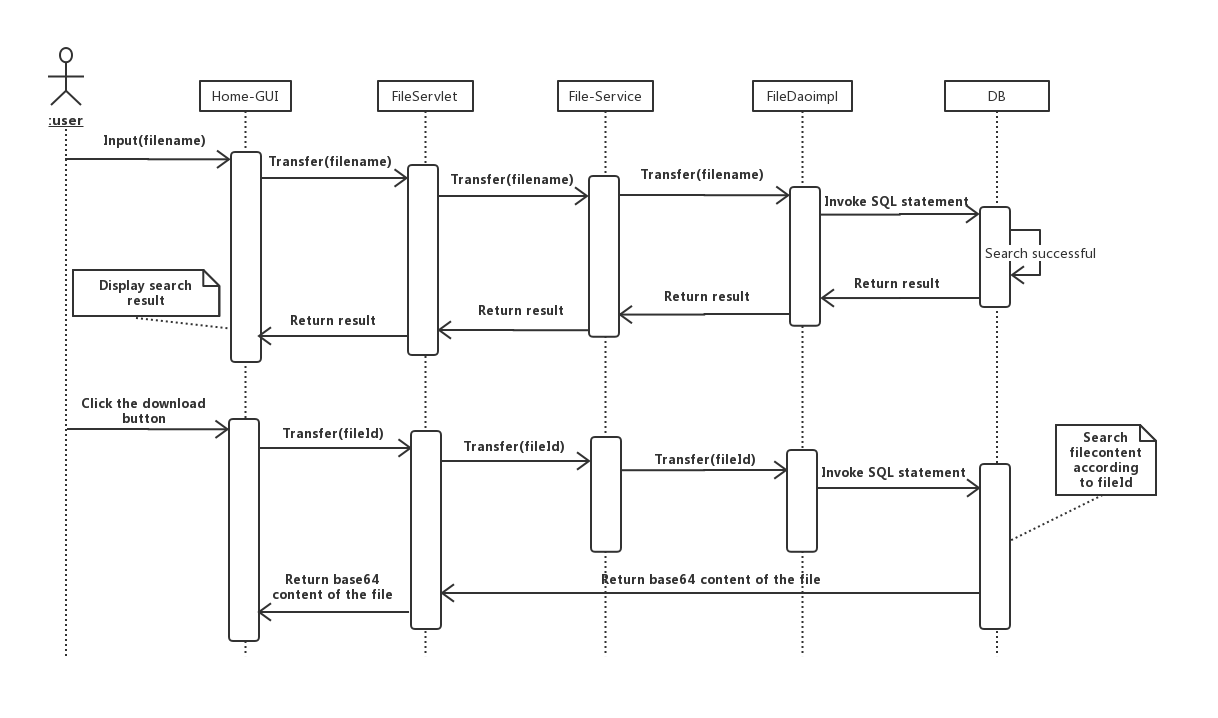
\includegraphics[scale=0.37]{Sequence_diagram_search_and_download.png}
\caption{Sequence diagram of search and download}
\label{fig:Sequence diagram of search and download}
\end{figure}

\begin{figure}[ht]

\centering
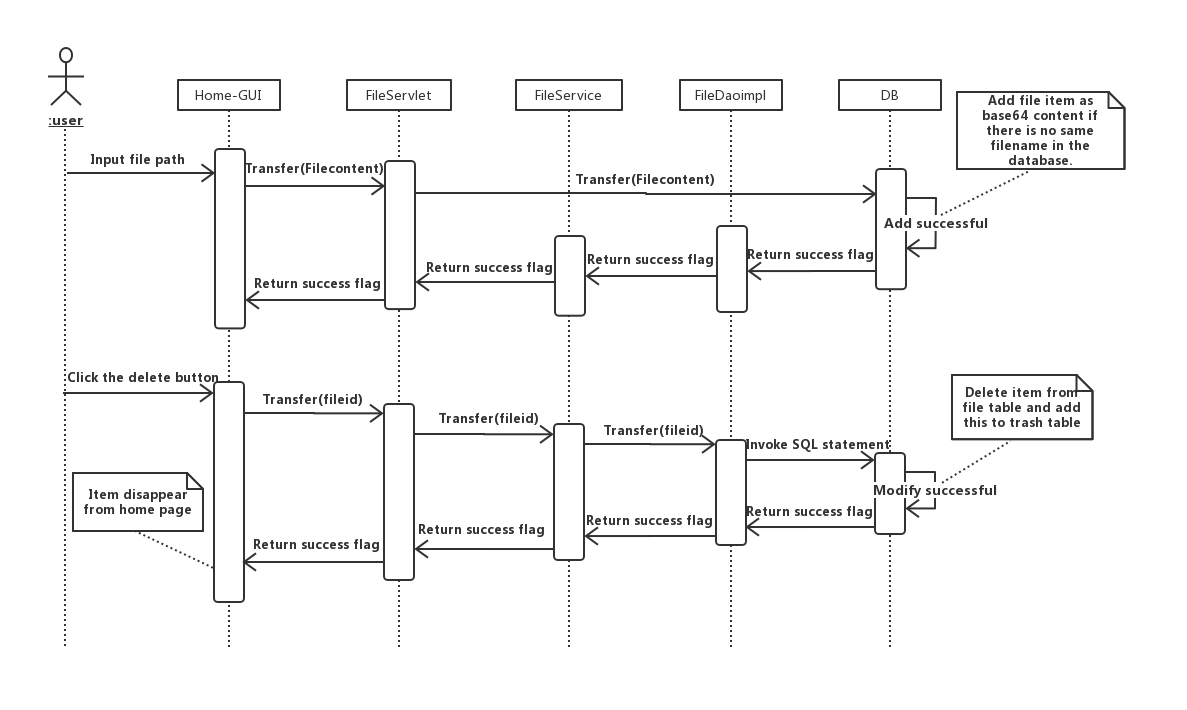
\includegraphics[scale=0.38]{Sequence_diagram_upload_and_delete.png}
\caption{Sequence diagram of upload and delete}
\label{fig:Sequence diagram of upload and delete}
\end{figure}

\par There are three tables in the database, namely users, file and trash. 

\par The users table has two attributes, name and pwd, representing the username and password, respectively. The attributes of the file table are u\_name (uploaded user name), name (filename), content, private (to indicate whether it is a private file or not), and lockval (indicates the locking status of the file), where the content is the full file content, stored in base64 format. The base64 formation of storing file content directly in the database is another way to increase security, considering that base64 can store file content implicitly and requires a password to access the database. However, the disadvantage is that such storage delay is relatively high, as well as increasing the amount of data. Both private and lockval are an integer of 1 bit. Private is 0 means the file is public while 1 means the user's private file. And lockval is 0 means the file is not locked while 1 means the file is locked or occupied. In the file table, name and private bonded together as the joint primary key, that is, name and private determine the only specific file.

\par The trash table has six attributes: id (naturally incremented id), u\_name (uploaded user name), name (filename), content, private (whether the file is private before deletion), and lockval (lock status of files in the trash). The id is used as the primary key in the trash table to identify a single trash file that is unique. Because there can be multiple files of the same name and possibly in different versions in the trash bin, set the id to the naturally incrementing primary key. Every time a new file is moved to the trash, the id of this file is automatically added by 1. The reason for adding lockval to trash is that there are always conflicts when the user operates in the trash, thus apparently it is necessary to lock the files in the trash.

\par The implementation of the server program is much more complex, and the dependencies and invocation relationships between classes can be seen in the class diagram (the figure 12 at the Appendix of the report).To summarize, there are two JavaBean types declared according to the main entity objects involved in the system: user and file, each containing some corresponding variables and corresponding constructor, getter and setter. The properties in the user class are simple, just the username name and password pwd. On the other hand, there are four attributes in the file class: uName(upload user name), name (file name), content(file content), and pri(public/private file identifier). Both beans involve many different operations, which leads to the subsequent fileDao and userDao interfaces, which declare all the methods to be used. The UserDaoImpl and FileDaoImpl implementation classes correspond to two interfaces, respectively. Both types of bean involve methods that have concrete implementations in the implementation class.

\par In order to increase the reusability of the code and keep the maximum flexibility, as the relay point between the servlet class and the interface implementation class, the service class is created, which is divided into userService and fileService to provide corresponding service (method) for the servlet class. All implemented interface methods will be invoked in the corresponding service class, so the number of methods in the service is the same as the number of methods in the DaoImpl class.

\par Then there are the two most complex classes: fileServlet and userServlet, which handle the various HTTP requests that come from the front end. The userServlet class primarily handles requests related to user information, while the fileServlet handles all requests related to file operations. Due to the complexity of the business logic, an example is given to illustrate the detailed business logic of the function. The report takes the most complex operation 'file recovery' as an example.

\par First, the parameters in the post request sent by the front end are action, id, pri and name. One thing to note is that the action is a parameter that is explicitly displayed in the URL for each request indicating the current action, which refers to 'recover' in this example. HTTP requests sent from the front end go through the filter first. There is no action in the filter and the sole purpose is to unify the encoding of the requests and responses going through the filter to UTF-8. The fileServlet class then intercepts the link, take and detect the action parameter of the request, and perform corresponding operations after recognizing it is 'recover'.
\begin{lstlisting}[language=Java]
}else if (action.equals("recover")) {
	String fName = req.getParameter("fname");
	String pri = req.getParameter("pri");
	String fID = req.getParameter("id");
    	JSONObject jsonObject = new JSONObject();
\end{lstlisting}
\par First extracts the parameters needed for the recovery operation -- the file name fname, the private value of the file, and the id of the file in the trash bin. The JSON object declared here is used to encapsulate the return information later. It is important to note that the system state is varied when restoring files and needs to be identified one by one and acted upon appropriately. The first thing to do is to the existFile() method to determine whether a current file exists in the system. The reason to do this is that if the current file is not present in the system, the program simply inserts the file information in the trash table back into the file table, whereas when the file is present in the system, a series of operations to overwrite the file are required.
\begin{lstlisting}[language=Java]
if(fileService.existFile(fName, Integer.parseInt(pri))) {   // if the file existed
	if(pri.equals("0")) {				//public file recover need both lock
		boolean flag =fileService.gainlock(fName);
		if(flag) {					//gain public lock
			flag =fileService.gainTrashlock(fID);
			if(flag) {				//gain trash lock
				flag = fileService.deleteFile(fName, Integer.parseInt(pri));
				if(flag) {
					flag = fileService.recoverFile(fID);
					if(flag) {
						jsonObject.put("ret", "0");
						jsonObject.put("msg", "Rollback success");
					}
					else {
						jsonObject.put("ret", "1");
						jsonObject.put("msg", "Rollback failed");
						System.out.println("releasing trash lock for "+fID);
						//release trash lock 
						flag = fileService.releaseTrashlock(fID);
						if(!flag) {
							jsonObject.put("ret", "1");
							jsonObject.put("msg", "fail to release trash lock");
						}
					}
				}
				else {
					jsonObject.put("ret", "1");
					jsonObject.put("msg", "delete failed");
				}
				
				
				//release public lock
				flag = fileService.releaselock(fName);
				if(!flag) {
					jsonObject.put("ret", "1");
					jsonObject.put("msg", "fail to release public lock");
				}
\end{lstlisting}
\par If the current file already exists in the system, we do a series of operations to overwrite the file. First, determine whether the file is public by the value of private. If it is a private file, the system only needs to lock the files in the trash bin, and do not need to lock the files with the same name in the public space at the same time -- there will be no conflict in the private space. The gainlock() method gets the public file lock, while the gainTrashlock() method gets the file lock in the trash. When a successful lock on a file determines that other users do not conflict with the current file operation, it is feasible to work with the data in the database.
Methods deleteFile() deletes the file in the public space and thus make room for the recovered file of the same name in the trash bin through method recover(), thus preventing the file table has data of the same primary key. At the end of the data recovery operation, the corresponding file lock in the trash bin and the file lock in the public space need to be released. Although the whole data of the file in the file table (including lockval) has been deleted, because the default value of lockavl is 1, when insert new data into the file table without giving specific lockval values, lockval is still 1, which shows that as the locked state, so the system still need to call releaselock() method to release the lock after executing the recovery operation. Meanwhile, there is no data of this file in the trash table and there is no need to release the lock. Only when recover fails does the system need to release the lock of the trash bin.
\begin{lstlisting}
else {							//private file only need trash lock
	boolean flag = fileService.gainTrashlock(fID);
	if(flag) {			// gain trash lock
		flag = fileService.deleteFile(fName, Integer.parseInt(pri));
		if(flag) {
			flag = fileService.recoverFile(fID);
			if(flag) {
				jsonObject.put("ret", "0");
				jsonObject.put("msg", "Rollback success");
			}
			else {
				jsonObject.put("ret", "1");
				jsonObject.put("msg", "Rollback failed");
				//release trash lock 
				flag = fileService.releaseTrashlock(fID);
				if(!flag) {
					jsonObject.put("ret", "1");
					jsonObject.put("msg", "fail to release trash lock");
				}
			}
		}
		else {
			jsonObject.put("ret", "1");
			jsonObject.put("msg", "delete failed");
		}
		
		
	}
	else {				//gain trash lock failed
		jsonObject.put("ret", "1");
		jsonObject.put("msg", "fail to gain trash lock");
	}
}
\end{lstlisting}

\par For private files, there will be no other user manipulating the same file at the same time, which means no conflict, so the system will only need the lock of the files in the trash bin and then execute the deleteFile() and recoverFile() methods. Similarly, the corresponding file lock in the bin is released only if the rollback fails. When this file does not exist in the system, similar to private file recovery, the system just needs to get the trash bin file lock, then execute deleteFile() and recoverFile() to completely delete the data in the bin or restore to public or private space. As mentioned earlier, when the new file information is inserted back into the file table, releaselock() needs to be called to change its laockval default value from 1 to 0 in case a subsequent user is unable to manipulate the file, as shown in the code below.
\begin{lstlisting}
else {							//no  to-be-recovered file exist
	boolean flag = fileService.gainTrashlock(fID);
	if(flag) {				//gain trash lock, no need for public lock
		flag = fileService.recoverFile(fID);
		if(flag) {				
				jsonObject.put("ret", "0");
				jsonObject.put("msg","recover success!");
				
				//release lock
				if(pri.equals("0")) {	   		//prevent pri from being default value "1"							
				 	flag = fileService.releaselock(fName);
				 	if(!flag) {
						jsonObject.put("ret", "1");
						jsonObject.put("msg", "rollback success but fail to release lock");
					}
			}
		}
		else {				//recover failed, need release trash lock
			jsonObject.put("ret", "1");
			jsonObject.put("msg", "recover failed");
			//release trash lock 
			flag = fileService.releaseTrashlock(fID);
			if(!flag) {
				jsonObject.put("ret", "1");
				jsonObject.put("msg", "fail to release trash lock");
			}
		}
}
	else {
		jsonObject.put("ret", "1");
		jsonObject.put("msg", "fail to gain trash lock");
	
	}
	
}
\end{lstlisting}
\par At the end of the operation, the JSON object is encapsulated into the response object and returned to the front end. The specific statement is as follows.
\begin{lstlisting}
resp.getWriter().write(jsonObject.toString());
return;
\end{lstlisting}
\par The above is the detailed process of recover operation, where the overall logical structure is showed in figure 11.
\begin{figure}[ht]

\centering
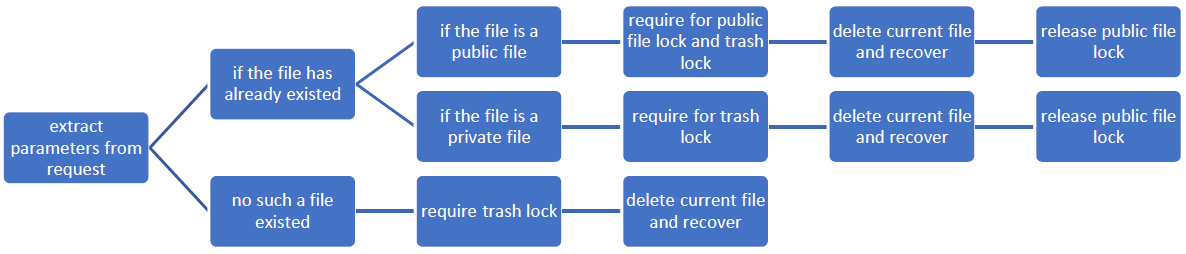
\includegraphics[scale=0.506]{logic.png}
\caption{Logic of recovery}
\label{fig:1}
\end{figure}
\subsection{Testing}
\begin{itemize}
\item UI: crucial button clear; error feedback normal; no redundant menu bar or link; concise and user-friendly interface; no picture cover or overlap.
\item Funtionality:
\begin{table}[H]
\centering
\setlength{\tabcolsep}{1.5mm}{
\begin{tabular}{|c|p{5cm}|p{5cm}|c|}
\hline
Function & Input value & Result or feedback & Achieve \\
\hline
\multirow{2}*{Login} & Correct username and password & Successful login & Yes  \\
\cline{2-4}
& Wrong username and password & User name or password error & Yes \\
\hline
\multirow{2}*{Registration} & Valid username and password & Successful register & Yes  \\
\cline{2-4}
& Invalid username and password & Failed register & Yes  \\
\hline
\multirow{2}*{Change password} & Correct previous username and password & Change password successfully & Yes  \\
\cline{2-4}
& Wrong previous username and password & Old password error & Yes  \\
\hline
Logout & / & Logout & Yes  \\
\hline
\multirow{2}*{Search by keyword} & Existing keyword & Show corresponding files & Yes  \\
\cline{2-4}
& Non-existing keyword & Show empty file list & Yes  \\
\hline
Clear & / & Clear searching content and back to public space list & Yes  \\
\hline
\multirow{2}*{Search by username} & Existing username & Show corresponding files & Yes  \\
\cline{2-4}
& Non-existing username & Show empty file list & Yes  \\
\hline
Access private space & / & Show private space list & Yes  \\
\hline
Upload to public & Select file to be uploaded & Upload successfuly & Yes  \\
\hline
Upload to pirvate & Select file to be uploaded and select private option & Upload successfuly & Yes  \\
\hline
Download & Select file to be downloaded & download successfuly & Yes  \\
\hline
Deletion & Select file to be downloaded & deleted successfuly & Yes  \\
\hline
Lock file & / & Other user cannot operate the files & Yes  \\
\hline
Overwrite file & / & File overwritten & Yes  \\
\hline
Recover file & Select file to be recovered & File recovered & Yes  \\
\hline

\end{tabular}}
\caption{Testing}
\end{table}

\item Security: No serious security vulnerabilities after OWASP scan. There exists the possibility of unauthorized page access jump. However, there is no access authority to the account or files after the jump, and system prompt error.
\end{itemize}

\section{Team work}
% Describe how you worked together, including the tools and processes you
% used to facilitate group work.
This project is quite a challenge for our team but we worked together well and successfully conquered it. At the very beginning of our project, we reached an agreement on the agile developing model and scrum approach which means we have a short-period working plan at each stage of our project.
\par The meetings are held regularly. Usually, there are 2 meetings each week. In addition, we use wechat for online discussion as well. On each face-to-face meeting we usually summarize the work of the previous time period and then we would argue with the core problems we encountered during the job, and at last, the targets would be set for the next round. As for online meetings, the scattered ideas and details are debated and many on-going jobs are done in time thanks to this real-time communication. It is necessary to mention that at the early stage of our project, our team used wechat very frequently but it was after that we realized that Github is a much better tool for coding. Thus we transferred plenty of our communication details to Github later.
\par Since Dropbox is our ultimate example and objective, during the exploration of it we found DropPaper which is a great tool for group working as well. Quite naturally, we adopt it as a recording tool for important files associated with our project like the meeting records or the newest version of our software, along with a lot of draft of course.
This project trains us on many aspects of abilities. For working with each other efficiently, our communication skills are improved. The work balancing is fairly vital to not let anyone bear too much work. Therefore, our work is periodically divided by one of our team members who are currently responsible for the part of work at the time. Besides, leadership is also important in group working. Because there is no particular leader during the project, everyone has to be a temporary leader for a period.  

\section{Evaluation}
% Critically evaluate your project: what worked well, and what didn’t? how
% did you do relative to your plan? what changes were the result of improved thinking
% and what changes were forced upon you? how did your team work together? etc. Note
% that you need to show that you understand the weaknesses in your work as well as its
% strengths. You may wish to identify relevant future work that could be done on your
% project.
Eventually, we accomplished approximately 80 per cent of our initial plan. This percentage is based on our backlog set in the initial report. 
\par The basic functions, which we have all successfully implemented in our system, includes a web and an Android app with user registration and login/logout, changing the password, file upload and download among multiple hosts. The more complex targets including public and private storing space, searching by username and keyword, file renaming, deletion to trash bin and recovery are also completed. Due to the automatically overwrite procedure, the system is synchronized. And finally, locks are added when there are concurrent operations.
\par The requirements which we failed to satisfy in time include adding a password to files, sharing files with URL and create new folders.
\par Somehow there are some of our requirements implemented in a different way from our original design. For example, we planned to design a function of sorting files by some kind of order, but we considered it later again and decided to implement it as searching by username and keyword.
\par As we mentioned in our initial report, security issue like encryption of the file system, data compressing through the file transportation(Rsync Algorithm) are the tricky parts of the project and not listed in our backlog. It turns out that we don't have enough time to consider these issues. However, they really are the crucial requirements in practice and thus make our project weak in facing attacks and lowering load balancing.
\par In conclusion, our project achieved the basic implementation of a file management system. The design of the public and private spaces allow clients to manage their files more flexible. Moreover, storing the data in the database in an implicit way makes our system safe against data leaking problem. On the aspect of synchronization, the system keeps the files up-to-date by automatically overwritten while the trash bin provides a way to recover the old versions, which is, in our opinion, a nice measure to make the system not only clean but robust. Considering the massive concurrent operations, which is a very normal issue nowadays, our group designed the locking mechanism by which the system can avoid errors to some extent and give users feedback on locking files. 
\par Obviously this system also has some deficiencies. It is necessary to mention we are unable to gain the memory access to the mobile phone thus cannot download files with our Android app. There are some general issues that are not concerned. First of all, concurrent file downloading is not allowed because of our locking mechanism, although it actually does not raise a system problem and should be allowed. Other than that, our system is not promising in data security through transmitting since the data are transmitted in clear text without any encryption.
\section{Peer assessment}
% In a simple table, allocate the 100 ‘points’ you are given to each team
% member. Valid values range from 0 to 100 inclusive. You may assign decimal values, but
% the entire points must add up to precisely 100. An exception will be made if the 100
% points are evenly divided between team members, where recurring decimals presented to
% 2 decimal places will be interpreted as if they added up to 100 (e.g. for 6 members it is
% acceptable for all students to be allocated precisely 16.66 points).
\begin{table}[H]
\centering
\begin{tabular}{|c|c|c|c|c|c|c|}
\hline
Member & Haonan Li & Zifei Fu & Jiashuo Li & Chen Ling & Wenhao Dai & Huikang Liu \\
\hline
Marks & 16.5 & 16.5 & 17 & 17 & 16.5 & 16.5\\
\hline
\end{tabular}
\caption{Assessment}
\end{table}

\section{Appendix}
\begin{figure}[ht]

\centering
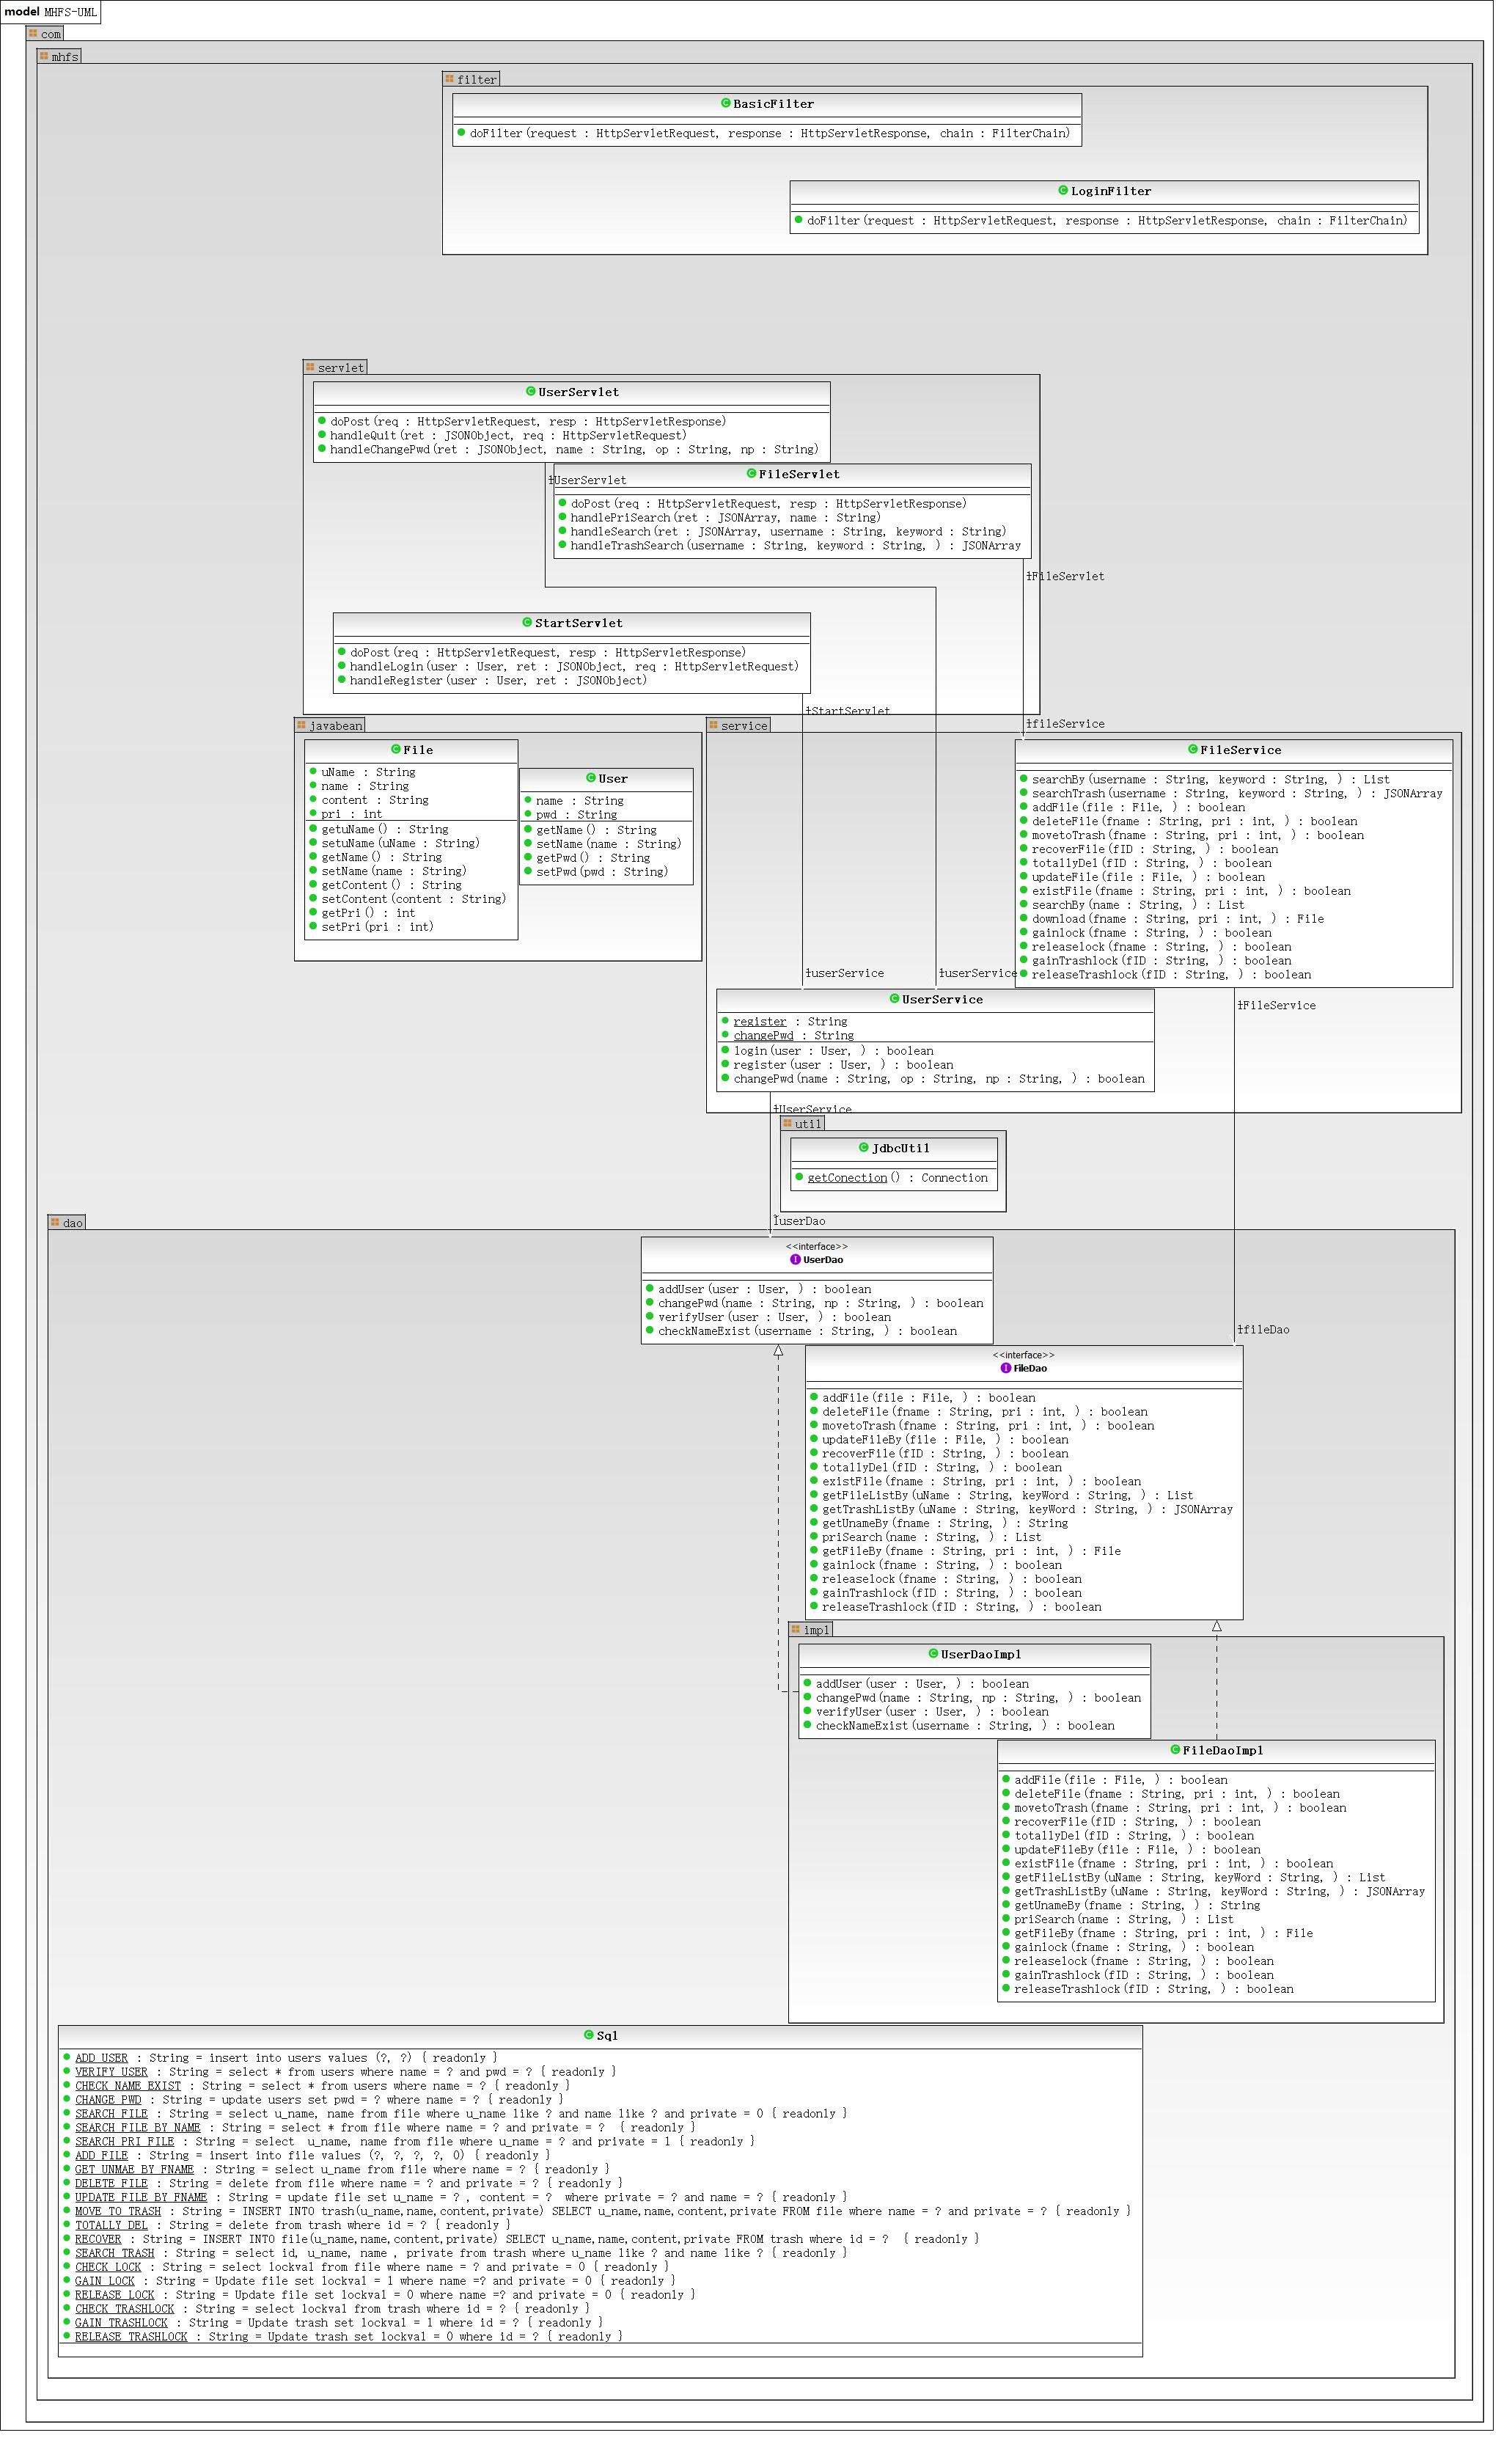
\includegraphics[width=16.5cm,height=21.5cm]{class.jpg}
\caption{class diagram}
\label{fig:2}
\end{figure}

\section{External Libraries}
\begin{itemize}
    \item bootstrap: https://getbootstrap.com/
    \item Android API 27 Platform: https://developer.android.google.cn
    \item json-20180813.jar: https://github.com/douglascrockford/JSON-java
    \item Java Platform (JDK) 1.8: https://www.oracle.com
    \item jQuery: https://jquery.com/
    \item java ee: https://www.oracle.com/technetwork/java/javaee/downloads/index.html
    \item Gradle: https://gradle.org
    \item JDBC driver: https://www.oracle.com/technetwork/database/application-development\\
    /jdbc/downloads/jdbc-ucp-183-5013470.html
\end{itemize}

\end{document}

